C++17带来了重要修改和几个与并发相关的调整,先让快速讨论一下后者。在C++11中引入的\texttt{std::lock()}现在有一个相应的RAII对象,\texttt{std::scoped\_lock}。添加了共享互斥锁\texttt{std::shared\_mutex},或者称为读写互斥锁(同样,匹配POSIX相应的特性)。只要线程不需要独占访问锁定的资源,这个互斥锁允许多个线程同时进行操作。这样的线程执行只读操作,而写线程需要独占访问,因此称为\textbf{读写锁}。理论上讲,这是一个聪明的想法,但大多数实现的性能都很糟糕。

值得注意的是一个新特性,允许决定L1缓存的缓存行大小,\texttt{std::hardware\_destructive\_\linebreak interference\_size}和\texttt{std::hardware\_constructive\_interference\_size}。这些常量有助于创建缓存优化的数据结构,避免错误共享。

现在来看看C++17的主要新特性——\textbf{并行算法},STL算法现在有了并行版本(总的来说,这组并行算法通常称为并行STL)。例如,下面是对\texttt{std::for\_each}的使用:

\begin{lstlisting}[style=styleCXX]
std::vector<double> v;
… add data to v … 
std::for_each(v.begin(), v.end(),[](double& x){ ++x; });
\end{lstlisting}

在C++17中,可以让标准库在可用的处理器上并行执行:

\begin{lstlisting}[style=styleCXX]
std::vector<double> v;
… add data to v … 
std::for_each(std::execution::par,
			v.begin(), v.end(),[](double& x){ ++x; });
\end{lstlisting}

并行版本的STL算法有一个新的第一个参数:执行策略。注意,执行策略不是单个类型,而是一个模板参数。该标准提供了几个执行策略,前面使用的并行策略\texttt{std::execution::par},允许算法在多个线程上执行。线程的数量和线程中计算分区的方式没有指定的,完全取决于实现。顺序策略\texttt{std::execution::seq}则是在单个线程上执行算法,与不使用任何策略(或在C++17之前)执行算法的方式相同。

还有一个并行的非串行策略,\texttt{std::execution::par\_unseq}。这两个并行策略之间有微妙的区别,理解这个区别很重要。标准表示无序策略允许在单个线程中交叉进行计算,从而允许进行其他优化,如向量化。但优化编译器在生成机器码时可以使用像AVX这样的向量指令,而且这无需任何来C++代码的帮助。编译器只是找到向量化的机会,并将常规的单字指令替换为向量指令。那这里有什么不同呢?

为了理解非串行策略的本质,必须考虑一个更复杂的例子。现在,不是简单地操作每个元素,想使用共享数据做一些计算:

\begin{lstlisting}[style=styleCXX]
double much_computing(double x);
std::vector<double> v;
… add data to v … 
double res = 0;
std::mutex res_lock;
std::for_each(std::execution::par, v.begin(), v.end(),
[&](double& x){ 
	double term = much_computing(x);
	std::lock_guard guard(res_lock);
	res += term;
});
\end{lstlisting}

这里对每个向量元素进行一些计算,然后累加结果的总和。计算本身可以并行完成,但是累加值必须由一个锁来保护,因为所有线程都会增加同一个共享变量\textit{res}。由于锁并行执行策略是安全的,但不能在这里使用无顺序的策略。如果同一个线程要同时处理多个向量元素(交叉处理),可能会多次尝试获取同一个锁,这是会产生死锁。如果线程持有锁,并试图再次锁定它,第二次尝试将会阻塞,并且线程不能继续运行到它应该解锁的地方。标准调用代码(如上一个例子中的\textbf{向量化不安全})声明,此类代码不应与无序策略一起使用。 

既然已经了解了并行算法在理论上是如何工作的,那么在实践中呢?简短的回答很好,但有一些瑕疵,还是来看看完整的版本。

检查并行算法之前,必须准备构建的环境。要编译C++程序只需要安装所需的编译器版本,比如GCC,然后就可以了,但并行算法却不是这样。在写这本书的时候,安装过程有些繁琐。

最新的GCC和Clang版本都包含了并行的STL头文件(在一些安装中,Clang需要安装GCC,因为它使用GCC提供的并行STL),这个问题出现在较底的层次上。这两个编译器使用的运行时线程系统是Intel的\textbf{threading Building Blocks (TBB)},这两个编译器都没有在安装中包含TBB。麻烦的是,编译器的每个版本都需要对应的TBB版本,旧版本和新版本都不能工作(错误会在编译和链接时出现)。要运行与TBB链接的程序,可能需要将TBB库添加到库路径中。

当解决了这些问题,并配置了编译器和必要的库,使用并行算法并不比使用其他STL困难。那么其扩展性怎么样?我们可以做一些基准测试。 

从\texttt{std::for\_each}开始,没有锁,并且每个元素都需要大量的计算(函数\texttt{work()}非常耗时,精确的操作对于扩展性并不重要):

\hspace*{\fill} \\ %插入空行
\noindent
\textbf{parallel\_algorithm.C}
\begin{lstlisting}[style=styleCXX]
std::vector<double> v(N);
std::for_each(std::execution::par,
v.begin(), v.end(),[](double& x){ work(x); });
\end{lstlisting}

以下是运行在两个线程上的串行版本和并行版本的性能:

%\hspace*{\fill} \\ %插入空行
\begin{center}
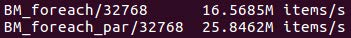
\includegraphics[width=0.9\textwidth]{content/2/chapter8/images/1.jpg}\\
图8.1 - 并行\texttt{std::foreach}在2个cpu上的基准测试
\end{center}

扩展性还不错。注意,向量大小N相当大,有32K个元素。对于更大的向量,扩展效果确实有所改善。但是,对于相对较小的数据量,并行算法的性能很差:

%\hspace*{\fill} \\ %插入空行
\begin{center}
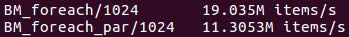
\includegraphics[width=0.9\textwidth]{content/2/chapter8/images/2.jpg}\\
图8.2 - 短序列并行\texttt{std::foreach}的基准测试
\end{center}

对于包含1024个元素的向量,并行版本比串行版本慢。原因是执行策略在每个并行算法开始时启动所有线程,并在结束时回收它们。启动新线程需要花费大量时间,因此当计算时间较短时,开销会超过我们从并行化中获得的任何加速。这不是标准强加的要求,而是当前GCC和Clang中并行STL的实现管理其与TBB系统交互的方式。 

当然,并行算法提高性能的大小取决于硬件、编译器,及其并行性的实现,以及每个元素的计算量。例如,可以尝试逐元素计算:

\begin{lstlisting}[style=styleCXX]
std::for_each(std::execution::par,
v.begin(), v.end(),[](double& x){ ++x; });
\end{lstlisting}

现在,处理32k元素数组,并行性并没有优势:

%\hspace*{\fill} \\ %插入空行
\begin{center}
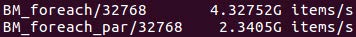
\includegraphics[width=0.9\textwidth]{content/2/chapter8/images/3.jpg}\\
图8.3 - 并行\texttt{std::foreach}的基准测试,以实现每个元素的快速计算
\end{center}

对于更大的数组,并行算法可能会有优势,除非内存访问速度限制了单线程和多线程版本的性能(这是一个很大的内存限制计算)。

也许更令人印象深刻的是那些很难并行化算法的性能,比如\texttt{std::sort}:

\begin{lstlisting}[style=styleCXX]
std::vector<double> v(N);
std::sort(std::execution::par, v.begin(), v.end();
\end{lstlisting}

输出:

%\hspace*{\fill} \\ %插入空行
\begin{center}
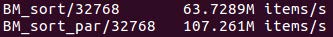
\includegraphics[width=0.9\textwidth]{content/2/chapter8/images/4.jpg}\\
图8.4 - 并行\texttt{std::sort}的基准测试
\end{center}

同样,在并行算法生效之前,需要足够大的数据量(对于1024个元素,单线程排序更快)。排序并不是容易并行化的算法,而且在双精度浮点数(比较和交换)上对每个元素进行的计算非常快。尽管如此,并行算法展示了非常好的加速,如果元素比较的代价更高,性能会变得更好。 

并行STL算法如何与线程交互?若在两个线程上同时运行两个并行算法会发生什么?首先,与在多线程上运行的代码一样,必须确保线程安全(无论使用哪种排序,在同一个容器上并行两个排序不个好主意)。除此之外,还会发现多个并行算法可以共存,但无法控制调度系统,它们都试图在可用的CPU上运行,因此会出现争夺资源。根据每个算法的扩展性,并行运行几个算法可能会获得更高的总体性能,也可能不会。

总的来说,当STL算法运行在足够大的数据量上时,其并行版本的性能非常好,尽管足够大的数据量取决于特定的计算。可能需要额外的库来编译和运行使用并行算法的程序,配置这些库可能需要一些工作量。而且,并不是所有的STL算法都有并行版本(例如,\texttt{std::accumulate}就没有)。

……

现在我们可以在穿梭时间,直接跳到C++20。














